\documentclass{article}
\usepackage{graphicx}
\usepackage{vmargin}
\usepackage{hyperref}
\usepackage{amsmath}
\usepackage{url}
\setpapersize{A4}
\setmarginsrb{2.5cm}{2.5cm}{2.4cm}{2.8cm}{12pt}{14pt}{12pt}{22pt}
\pagestyle{empty}

%%% define \maketitle without the vertical space %%%
\makeatletter
\def\@maketitle{%
  \newpage
%  \null% DELETED
%  \vskip 2em% DELETED
  \begin{center}%
  \let \footnote \thanks
    {\LARGE \@title \par}%
    \vskip 0.75em%
    {\large
      \lineskip .5em%
      \begin{tabular}[t]{c}%
        \@author
      \end{tabular}\par}%
    \vskip 0.75em%
    {\small \@date}%
  \end{center}%
  \par
  \vskip 1.5em}
\makeatother
%%% reduce spacing between items in lists %%%
\newlength{\wideitemsep}
\setlength{\wideitemsep}{.5\itemsep}
\addtolength{\wideitemsep}{-7pt}
\let\olditem\item
\renewcommand{\item}{\setlength{\itemsep}{\wideitemsep}\olditem}
%%% reduce size of $\sim$ for use with bash paths %%%
\newcommand{\ttsim}{\raise.17ex\hbox{$\scriptstyle\mathtt{\sim}$}}
%%% define how bash code will be displayed (indented, preceded by '#' %%%
\newcommand{\shellcmd}[1]{\indent\indent\texttt{\small\# #1}\\}
%%%
\newcommand{\An}{\textit{Astrometry.net}}

\title{Palomar 200" LFC Reduction Cookbook}
\author{Micaela Bagley}
\date{December 2014}

\begin{document}
\maketitle

\section{Introduction}
This describes a set of Python codes that are written for the purpose 
of reducing imaging data observed with the Large Format Camera (LFC) on the 
200" at Palomar Observatory. This Cookbook explains how to reduce the data,
fit them with WCS solutions, stack the images, calibrate the photometry,
and create a final catalog of sources matched to the WISP catalogs.

\vspace{4 mm}
\section{Requirements}
Untar the directory of Python scripts in a convenient directory: 

\texttt{unzip palomarLFC.zip} \\
Add the following to your \ttsim/.bashrc and source it:

\texttt{export PYTHONPATH="\$PYTHONPATH:[path\_to\_scripts]/palomarLFC/"}

\texttt{export PATH="\$PATH:[path\_to\_scripts]/palomarLFC/"}\\

\noindent The following Python packages are required and can be installed 
automatically by running:

\texttt{pip install -r requirements.txt}
\begin{itemize}
\item \texttt{numpy}
\item \texttt{pyraf} (requires \texttt{IRAF})
\item \texttt{astropy}
\item \texttt{scipy}
\item \texttt{matplotlib}
\item \texttt{PyPhot}\footnote{Some of the IDL AstroLib photometry algorithms translated to Python. Written by David Jones, Johns Hopkins University}
\end{itemize}

\noindent Additional requirements:
\begin{itemize}
\item \texttt{astrometry.net} (see below)
\item \texttt{Source Extractor}
\end{itemize}


\vspace{3 mm}
\section{Reduction}
\subsection{Organize the data}
The first step is to sort the data from a night of observations. 
The \texttt{extract\_header} module in \texttt{sort\_images.py} will
produce a file listing all images in a directory as well as their
image type, object name, exposure time, filter, airmass, and binning 
($1\times1$ or $2\times2$).\\

\texttt{usage: sort\_images.py [-h] dir} \\

\texttt{dir} $-$ \hangindent=2.7cm the directory for which to extract
information from all image headers.\\

\noindent You should have a directory for each night of science data (e.g.
\texttt{23mar12/}) and a directory for each of the types of calibration 
images to be used in reducing the science data (a directory each for 
biases, flats, and if necessary, darks). The directories for calibration 
images may be wherever you like (inside the
directory of science images, some random place on your computer, etc.)
as long as the calibration files have their own directories. \\

\noindent Inspect all calibration images and put any biases you don't 
want to use inside a directory called \texttt{unused/} within the biases 
directory. The same goes for the flats (and darks). The naming convention
for directories is necessary if you wish the reduction pipeline to 
automatically produce a log file. 

\subsection{Reduce a night of data}
\texttt{run\_reduction.py} is the wrapper for all reduction modules. There 
are several arguments and options available.

\hangindent=3cm \texttt{usage: reduction.py [-h] [--biasdir BIASDIR] 
    [--darkdir DARKDIR] [--flatdir FLATDIR] [--SaveSteps] 
    [--LogSteps LOGSTEPS] [--DarkSubtract] [--UseBias USEBIAS] 
    [--UseDark USEDARK] [--UseFlat [USEFLAT [USEFLAT ...]]] directory binning}\\

\texttt{directory} $-$ Directory to be reduced. Ex: 23mar12\\

\texttt{binning}~~ $-$ Binning of data to be reduced. ('binned' or 
    'unbinned')\\

\texttt{--biasdir BIASDIR} $-$ Directory containing the biases. 
    Default is \texttt{biases/}.\\

\texttt{--darkdir DARKDIR} $-$ Directory containing the darks. 
    Default is \texttt{darks/}.\\

\texttt{--flatdir FLATDIR} $-$ Directory containing the flats. 
    Default is \texttt{flats/}. \\

\texttt{--Overwrite} $-$ \hangindent=3.1cm Overwrite files after each 
     reduction step. If not set, images are saved as separate files, with
     strings ('bs', 'ds', 'ff') appended to  
     filenames to indicate reduction steps taken. \\

\texttt{--LogSteps LOGSTEPS} $-$ \hangindent=4.6cm Create a log file to 
    record the creation of calibration files and the science images 
    included in reduction. \\

\texttt{--DarkSubtract} $-$ Dark subtract the data. Dark subtract is not
    performed by default.\\

\texttt{--UseBias USEBIAS} $-$ Use a previously-created Master Bias. \\

\texttt{--UseDark USEDARK} $-$ Use a previously-created Master Dark. \\

\texttt{--UseFlat} $-$ Use a previously-created Master Flat. List a 
                       Flat for as many filters as necessary. \\

\noindent Paths to the directories containing the calibration files
should be \textit{relative} paths.
For example, consider a three night observing run in March of 2012. 
All data for this run are in a directory called \texttt{march2012/},
and we wish to reduce the data in \texttt{march2012/23mar12/}.
Biases and flats from this run are in \texttt{march2012/bias/}
and \texttt{march2012/flats/}, respectively.\\

\noindent To reduce binned data and output a logfile called 
\texttt{23mar12.log}:

\begin{quote}
\texttt{run\_reduction.py --biasdir march2012/bias/ --flatdir march2012/flats 
--LogSteps \\
march2012/23mar12.log march2012/23mar12 binned}
\end{quote}

\noindent Combined calibration images (e.g. \texttt{Bias\_unbinned.fits},
\texttt{Flatg\_unbinned.fits}) are written to their respective directories.
To reduce unbinned data, use a previously-created Bias, and output
a log file:
\begin{quote}
\texttt{run\_reduction.py --UseBias march2012/bias/Bias\_unbinned.fits --flatdir 
march2012/flats --LogSteps march2012/23mar12.log march2012/23mar12 unbinned} \\
\end{quote}

\noindent To reduce binned data, use previously-created Bias and Flats,
and output a log file (if there is more than one flat, list each flat that 
you want to use separated by a space):
\begin{quote}
\texttt{run\_reduction.py --UseBias march2012/bias/Bias\_binned.fits --UseFlat \\
march2012/flats/Flatg\_binned.fits march2012/flats/Flati\_binned.fits 
--LogSteps\\ ../march2012/23mar12.log march2012/23mar12 binned}
\end{quote}


\vspace{3 mm}
\section{Astrometry \& Alignment}
After reducing the data, sort all images by WISP parallel field with
one field per directory. Output files will be named after the directory.
For example, images in \texttt{Par300/} will be aligned and combined
to form \texttt{Par300\_[filter].fits}.
There are several fields that were observed on multiple nights. To avoid 
overwriting files, give each FITS file a unique name 
(include the date observed, for example). \\

\noindent Astrometry and image alignment is performed in $4$ steps:
\begin{enumerate}
\item \texttt{astrometrynet.py}
\item \texttt{fix\_astrometry.py}
\item \texttt{combine.py}
\item \texttt{align\_images.py} ~~(\texttt{imalign.pro})
\end{enumerate}
\subsection{\texttt{astrometrynet.py}}
The first step is to get a rough (though very good) approximate WCS 
solution for each image in a WISP parallel field using the \An~software 
package. \texttt{astrometry.py} builds the command that will
run the \An~software on each image in a directory. \\

\texttt{usage: astrometrynet.py [-h] [--useSE] wispfield} \\

\texttt{wispfield} $-$ \hangindent=2.7cm the WISP parallel field whose images
are to be fit with WCS solutions. This must match the name of the directory that
contains all relevant FITS files.\\

\texttt{--useSE} ~~$-$ \hangindent=2.7cm option to use \textit{SExtractor} 
to detect sources in each image rather than \An's bundled ``images2xy'' 
program. \\

\noindent Solved files are renamed \texttt{<base>\_solved.fits}. These 
are the original FITS images with headers updated to contain the WCS
solutions. 
The original FITS image as well as all of \An's auxiliary
output files are moved to a directory called \texttt{astrometric\_solns}.
See Appendix \ref{Anoutputs} for a list of the output files. \\

\noindent \An~software can take a long time if it must run 
through every available index file in order to find one that covers the
image. In order to expedite the process, \texttt{astrometrynet.py} tells \An~to:
\begin{itemize}
    \item skip running the FITS files through a ``sanitizer'', which cleans up
    non-standards-compliant images
    \item query only index files within 1$^{\circ}$ of the RA and Dec in the 
    image headers
    \item expect image pixel scales in the range $0.1 - 0.45$''/pix 
\end{itemize}
The range in the last step is enough to cover both binned and unbinned images
and ensures that only index files of the proper scale are used in 
determining the fit. (This step probably does not affect much as
that's a rather large range.) \\

\noindent \texttt{astrometrynet.py} prompts you to check your 
\texttt{/tmp} directory for any \texttt{[tmp.sanitized.*]} files.
\An\ can create loads of these files if it runs into any problems solving
for an image. \texttt{/tmp} is hard-wired into \An, but \texttt{/tmp} 
is pretty small on the physics network. \\

\subsection{\texttt{fix\_astrometry.py}}
The \An~software does a great job with the astrometry near the 
center of the chip. Most WISP fields
were observed on the top $1/3$ of the chip. At the bottom and edges of 
the images, the WCS gets further off. 
\texttt{fix\_astrometry.py} uses IRAF's CCMAP task to calculate
a second order solution that takes care of the small 
distortions and rotations at the edges. To do so, it compares the 
positions of objects in the Palomar images with those in the SDSS
catalog. Download the SDSS catalog in fits format\footnote{Download 
the catalog from
\url{http://skyserver.sdss3.org/dr10/en/tools/search/radial.aspx} in 
fits format} and put it in the directory \texttt{wispfield}. 
The LFC detector covers a lot of area, so a search
radius of 5 arcmin (or more) is best. 
\texttt{fix\_astrometry.py} expects the file to be called 
\texttt{result.fits}. \\

\noindent This script uses an IRAF task. Create a symbolic 
link to your \texttt{login.cl} file before running 
\texttt{fix\_astrometry.py}. \\

\texttt{usage: fix\_astrometry.py [-h] wispfield} \\

\texttt{wispfield} $-$ \hangindent=2.7cm the WISP parallel field whose images
are to be fit with improved WCS solutions. This must match the name of 
the directory that contains all relevant FITS files.\\

\texttt{Required files}: \\
\indent \indent \texttt{result.fits} $-$ the SDSS
catalog %\footnote{Download the catalog from 
%\url{http://skyserver.sdss3.org/dr10/en/tools/search/radial.aspx} in fits
%format} 
for the WISP field. \\

\noindent \texttt{fix\_astrometry.py} first runs \textit{SExtractor}
on all images and outputs a catalog and segmentation map named
\texttt{<base>\_astr\_cat.fits} and \texttt{<base>\_astr\_seg.fits},
respectively. For each image, it then matches the sources detected in the
Palomar image with the SDSS catalog. A file to be used with CCMAP, 
\texttt{SDSS.match}, is created
listing the Palomar $x,y$ coordinates with the SDSS RA and Dec for each 
source. Finally, it launches CCMAP, which allows the user to interactively
delete obvious residuals in the astrometric solution. The 
\texttt{<base>\_solved.fits} headers are updated with the new and 
improved WCS. 

\subsection{\texttt{combine.py}}
Once all images have corrected WCS solutions, images from like filters
are stacked using IRAF's IMCOMBINE task. Before combining, the user should
inspect all images and remove any for which the seeing is significantly worse.
Use IRAF's IMEXAM to check the FWHM of a few point sources across each image.
Make sure to check the observing logs as well for any mention of clouds or 
other problems. \texttt{combine.py} will prompt the user to stop and 
perform this inspection if they haven't already. \\

\texttt{usage: combine.py [-h] [--rejection {none,minmax,ccdclip,crreject,sigclip,avsigclip,pclip}] \\
\indent \indent \indent \indent \indent \texttt{[--combine {average,median,sum}] wispfield}} \\

\texttt{wispfield} $-$ \hangindent=2.7cm the WISP parallel field for which 
to stack image. This must match the name of the directory that contains all
relevant FITS files.\\

\texttt{--rejection} $-$ \hangindent=2.7cm the rejection algorithm to use. 
Default is \texttt{crreject}, which rejects only positive pixels and is 
appropriate for cosmic ray rejection. \\

\texttt{--combine} ~~$-$ \hangindent=2.7cm the type of combining operation 
to perform. Default is \texttt{median}. \\

\noindent See the IMCOMBINE help page for more information about parameter 
options.

\noindent For each filter, \texttt{combine.py} determines which images
need to be combined and prepares all parameters and files for use with 
IMCOMBINE. Multiplicative scale factors are calculated for each image
from the airmass (\texttt{[wispfield]\_[filter].scale}). 
The scale factor $=10^{0.4 ~ \kappa_F~ X}$, where $\kappa_F$ is the airmass 
coefficient calculated for the Palomar site\footnote{Taken from 
\url{http://www.ifa.hawaii.edu/~rgal/science/dposs/ccdproc/ccdproc_node3.html}, 
where $\kappa_g = -0.152$, $\kappa_r=-0.094$, and $\kappa_i=-0.07$.} 
and filter $F$.
Additive zero level shifts are calculated from the median value for 
each image. All zero corrections are done with respect to the first image,
so the images are sorted such that the lowest sky is listed first.  \\

\noindent The readnoise is necessary for IMCOMBINE's sigma clipping routines,
and can be estimated by binning the counts from an averaged bias frame. The
mean of the resulting histogram is the bias offset and 
the width of the distribution is $\sigma_{ADU} =~$readnoise/gain$~=~$FWHM.
The user should include in each WISP field directory the master bias from
each night the field was observed, and \texttt{combine.py} will estimate
an average readnoise to use for all images.\\

\noindent Finally \texttt{combine.py} reports the number of images available
in each filter and asks the user to choose the number of low/high pixels
to reject or the number of pixels to keep 
(depending on the rejection algorithm used). \\

\noindent IMCOMBINE uses the WCS in the headers to calculate and apply 
offsets to each image so they are properly aligned before stacking. 
Combined images are called \texttt{[wispfield]\_[filter].fits}. 
Sigma images are also created (\texttt{[wispfield]\_[filter]\_sig.fits}),
and the log file for the combination is called
\texttt{[wispfield]\_imcombine.log}. \\

\subsection{\texttt{align\_images.py}}
If there are 2 filters observed that night, \texttt{combine.py} will 
import \texttt{align\_images.py} to align those images using 
the WCS in the headers and IRAF's 
task WREGISTER.

\vspace{4 mm}
\section{Calibration}
For each field, the Palomar photometry is calibrated against the SDSS catalog 
(\texttt{result.fits}). \texttt{calibrate\_sdss.py} calculates both a zero 
point shift and a color term and saves them for use in calibrating the final 
catalog. \\

\texttt{usage: calibrate\_sdss.py [-h] wispfield} \\

\texttt{wispfield} $-$ \hangindent=2.7cm the WISP parallel field for which
to calibrate photometry. This must match the name of the directory that
contains all relevant FITS files.\\


\noindent \textit{SExtractor} is run in dual image mode
on the combined Palomar images with 
$1\sigma$ detection and analysis thresholds and a minimum area for 
detection of 5 pixels. Such low thresholds are used to ensure that as much
light as possible is included in each source's automatic magnitude. The 
Palomar catalogs are then match with the SDSS catalog using a $0.5''$
matching threshold. \\

\noindent The zero point shift, $zp = m_{SDSS} - m_{Palomar}$ 
is calculated for all sources, and those outside of $68\%$ of the
mean $zp$ are excluded. There is a residual slope visible in a plot of 
$zp$ that depends on color (top two rows of Fig.~\ref{fig:cals}).
This dependence is especially prevalent in the $g$ band.
Color terms to correct for this dependence 
are determined by fitting a line to the array of 
zero point shifts. Outliers (plotted in red) that are too far from the 
line in the 
$y$-direction are removed, and a new line (plotted in black) 
is fit to the remaining points. \\

\noindent The Palomar photometry is then calibrated by:\\
\indent $m_{calibrated} = m_{Palomar} + \alpha_0~(g-i)_{Palomar} + \alpha_1$,

\noindent where $\alpha_0$ is the slope of the best-fit line (the color term)
and $\alpha_1$ is the offset (the zero point shift). Several plots
are then created to check the quality of the calibration (rows $3-4$ in 
Fig.~\ref{fig:cals}). The last row shows the residuals of the calibrated 
data. For perfectly calibrated photometry, there would be no remaining
color dependence and the solid line would have a slope of zero.

\subsection{1 Palomar Filter, 1 WFC3 filter}
Fields that were observed with only one SDSS filter require a second
filter for determination of the color terms. For this we use the WFC3
UVIS filters that are available for the field. Possible color combinations
include ($g-$F814W), (F606W$-i$), ($g-$F600LP), and (F475X$-i$).
Use \texttt{calibrate\_sdss\_hst.py} in place of 
\texttt{calibrate\_sdss.py}.

\begin{figure}
\begin{center}
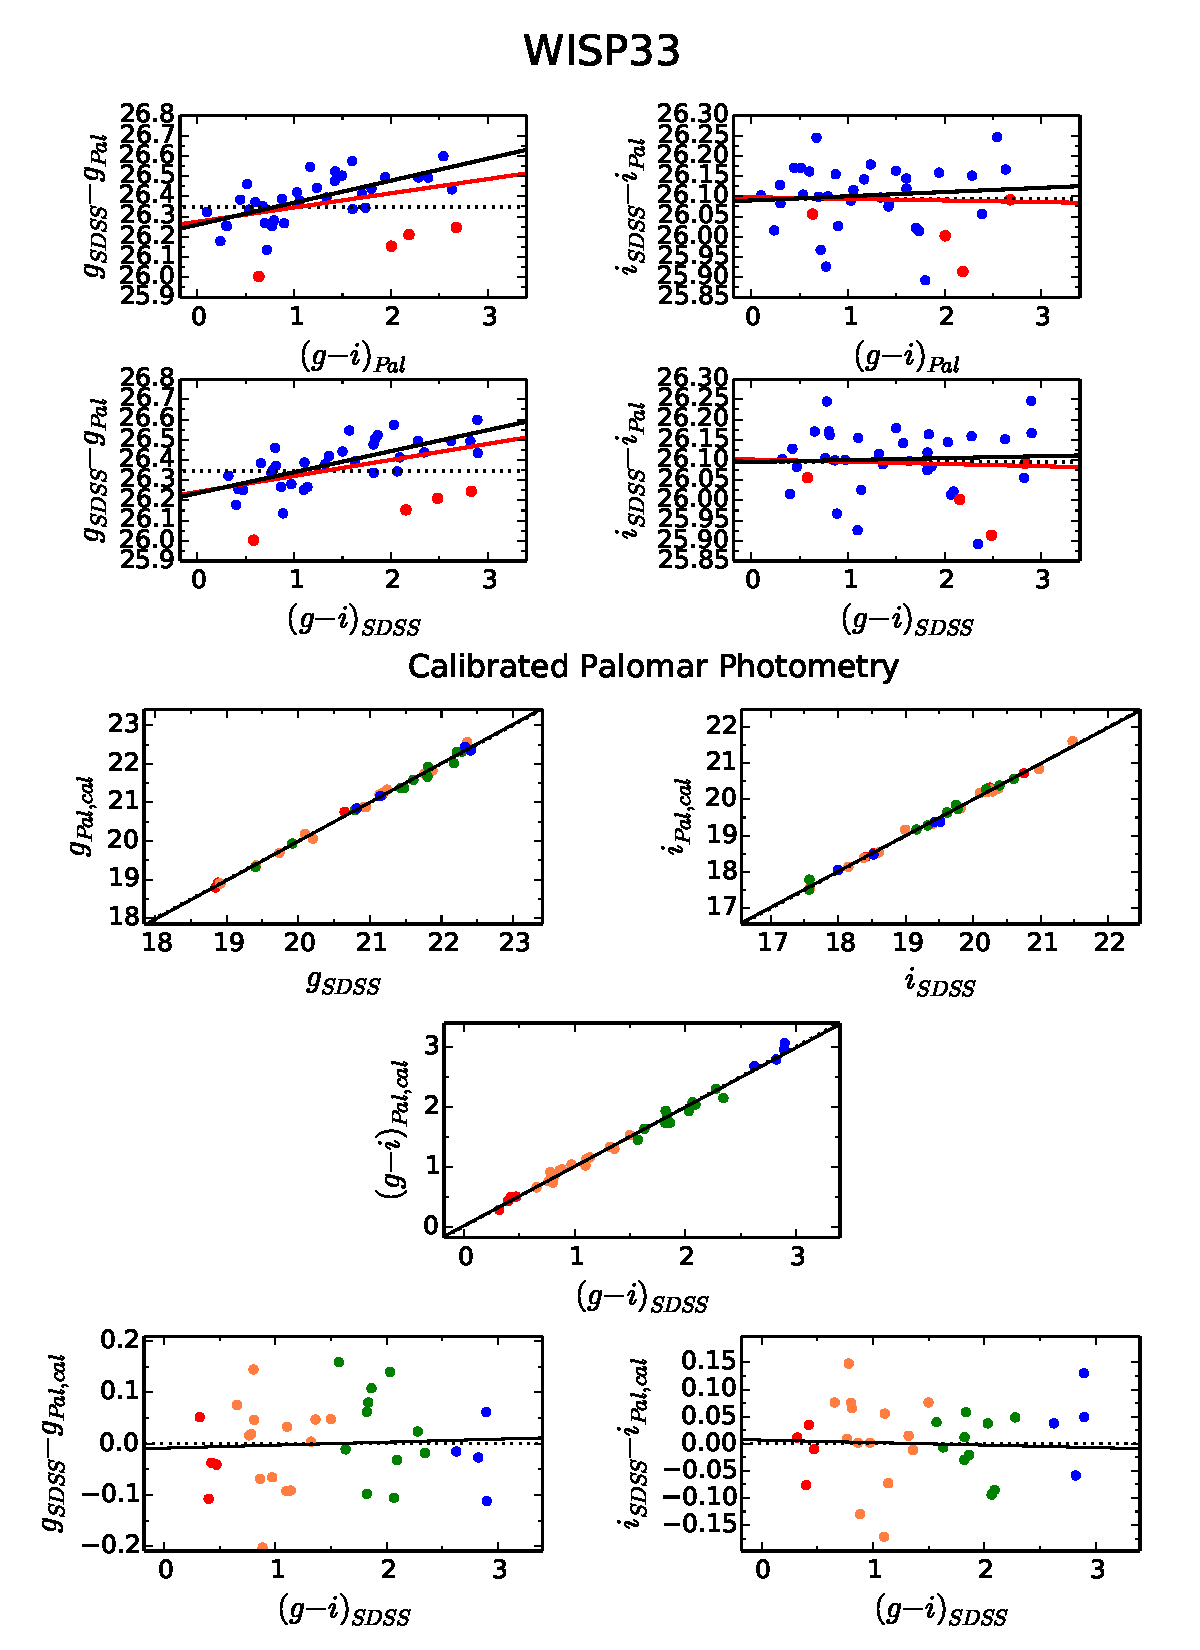
\includegraphics[scale=0.8]{sdss_calibration.pdf}
\caption{An example set of plots created by \texttt{calibrate\_sdss.py}
used to check the quality of the calibration. Zero point
shifts as a function of Palomar instrumental color (top row) and SDSS color 
($2^{nd}$ row). In the bottom three rows, points are color-coded by their
SDSS ($g-i$) color. The bottom row shows the residuals of the calibrated
photometry.
\label{fig:cals}
}
\end{center}
\end{figure}

\vspace{4 mm}
\section{Final Catalog}
\texttt{make\_final\_catalog.py} runs \textit{SExtractor} a final time
with detection and analysis thresholds of $2.2\sigma$ so that all sources
are detected at $\geq5\sigma$. The zero point shift and color terms 
calculated by \texttt{calibrate\_sdss.py} are applied to all Palomar
photometry. Palomar sources are matched to the WISP catalog with a 0.5''
matching radius. The final catalog includes both Palomar and WISP
RA and Dec and photometry from all available filters.\\

\texttt{usage: make\_final\_catalog.py [-h] wispfield} \\

\texttt{wispfield} $-$ \hangindent=2.7cm the WISP parallel field for which
to construct the final catalog. This must match the name of the directory that
contains all relevant FITS files.\\

\vspace{4 mm}
\appendix
\section{Installing \An}
Designate a directory for installation of \An~and its requirements.
In the following example, the installation directory is
\texttt{/home/bagley/Software}. \\

\noindent (Thanks to Michael Gordon (UMN-MIfA) for these installation 
instructions, which are also provided as a text file (\texttt{astro\_setup.txt})

\subsection{CFITSIO}
CFITSIO is a library of C and Fortran subroutines for reading and writing
data files in FITS data format, available from NASA's High Energy
Astrophysics Science Archive Research Center (HEASARC). 

\shellcmd{mkdir \ttsim/Software/cfitsio}
\shellcmd{cd \ttsim/Software/cfitsio}
\shellcmd{wget ftp://heasarc.gsfc.nasa.gov/software/fitsio/c/cfitsio\_latest.tar.gz}
\shellcmd{tar xzvf cfitsio\_latest.tar.gz}
\shellcmd{cd cfitsio}
\shellcmd{./configure --prefix=/home/bagley/Software/cfitsio}
\shellcmd{make}
\shellcmd{make install}

\noindent Add the following to your \ttsim/.bashrc and source it: \\
\shellcmd{export PKG\_CONFIG\_PATH=/home/bagley/Software/cfitsio/lib/pkgconfig}

\noindent Run the following commands, if they print something, you're good: \\
\shellcmd{pkg-config --cflags cfitsio}
\shellcmd{pkg-config --libs cfitsio}

\subsection{\An}
If you are running Python in a Virtual Environment, make sure you are 
in your virtualenv before completing the next steps. \\
\shellcmd{mkdir \ttsim/Software/astrometry}
\shellcmd{cd \ttsim/Software/astrometry}
\shellcmd{wget http://astrometry.net/downloads/astrometry.net-0.46.tar.bz2}
\shellcmd{tar xjvf astrometry.net-0.46.tar.bz2}
\shellcmd{cd astrometry.net-0.46}
\shellcmd{make}
\shellcmd{make py}
\shellcmd{make extra}
\shellcmd{make install INSTALL\_DIR=/home/bagley/Software/astrometry}

\noindent Add the following to your \ttsim/.bashrc and source it: \\
\shellcmd{export PATH="\$PATH:/home/bagley/Software/astrometry/bin"} 

\noindent In your virtualenv, run astrometry.net as: \\
\shellcmd{solve-field --no-plot img.fits .....}

\subsection{Index Files}
\An~requires index files, processed from an astrometric reference
catalog such as USNO-B1 or 2MASS. Pre-cooked index files built from the 
2MASS catalog are available \htmladdnormallink{here}
{http://data.astrometry.net/4200}. Use the \texttt{wget} script to download
the full catalog of index files, requiring about 10G of space. Alternatively, 
use the healpix png's to determine in which tiles your fields of interest
reside and download only the relevant index files. \\

\noindent The software looks for index files in 
\texttt{\ttsim/Software/astrometry/data}. If you don't have enough space
there, symlimk the \texttt{data} directory to their actual location. \\
\shellcmd{cd \ttsim/Software/astrometry}
\shellcmd{rmdir data}
\shellcmd{ln -s /other/thing/data data}

\section{\An~Default Outputs}\label{Anoutputs}
\[ \begin{array}{lcl}
\mbox{\texttt{<base>.wcs}} & - & \mbox{a FITS WCS header for the solution} \\
\mbox{\texttt{<base>.new}} & - & \mbox{a new FITS file containing the WCS header (renamed \texttt{<base>\_solved.fits})} \\
\mbox{\texttt{<base>-indx.xyls}} & - & \mbox{a FITS BINTABLE with the pixel locations of stars from the indx} \\
\mbox{\texttt{<base>.rdls}} & - & \mbox{a FITS BINTABLE with the Ra,Dec of sources extracted from the image} \\
\mbox{\texttt{<base>.axy}} & - & \mbox{a FITS BINTABLE of the sources extracted, plus headers that describe the job} \\
\mbox{} & & \mbox{(how the image is going to be solved)} \\
\mbox{\texttt{<base>.corr}} & - & \mbox{a basic FITS header} \\
\mbox{\texttt{<base>.solved}} & - & \mbox{exists and contains (binary) 1 if the field solved} \\
\mbox{\texttt{<base>.match}} & - & \mbox{a FITS BINTABLE describing the quad match that solved the image}
\end{array}\]

\noindent These may be useful if the user ever wishes to check the WCS
solutions. To keep \An~from creating these files, add \texttt{--wcs `none'},
etc., to the command. Output options are:
\texttt{--wcs}, \texttt{--new-fits}, \texttt{--keep-xylist},
\texttt{--rdls}, \texttt{--pnm}(?), \texttt{--corr},
\texttt{--solved}, \texttt{--match}, respectively. (I have not tried 
suppressing the creation of these files. See \An's README for more 
information.)


\end{document}
